\section{Introduction}
\label{sec:introduction}

Large language model (LLM)-based multi-agent systems (MAS) have become a promising paradigm for solving complex tasks.
By assigning planning, reasoning, execution, and verification to specialized agents, MAS decompose difficult problems into coordinated sub-processes and combine the complementary capabilities of multiple LLM calls
\citep{wu2023autogen,li2023camel,chen2023agentverse,yao2024multiagent}.
Their effectiveness, however, depends not only on the underlying language models and workflow topology, but also on the prompts that govern individual agents.
Prompts determine how an agent interprets its role, consumes upstream information, and communicates with downstream agents.
Consequently, optimizing prompts has become a key mechanism for improving the performance of a fixed multi-agent system.

Prompt optimization in MAS is substantially more challenging than in a single-agent setting.
Different agents solve different sub-problems and therefore require role-specific instructions, while their behaviors remain strongly coupled through inter-agent communication.
A change to an upstream prompt can alter the input distribution seen by several downstream agents, making an individually improved prompt potentially harmful to the overall workflow.
Moreover, the appropriate instruction for an agent may depend on the execution state reached by a particular task.
An instruction that is useful early in a trajectory may become irrelevant or even counterproductive after new evidence, tool outputs, or execution failures emerge.
This suggests a more desirable form of prompt optimization in which prompts are not treated as immutable parameters of an episode, but can adapt to the evolving state of the task.

Existing MAS prompt optimization approaches can be broadly grouped into two paradigms.
The first optimizes prompts for individual agents using local feedback or generic prompt optimizers.
Such methods are simple and effective, but they largely ignore dependencies among agents.
The second performs system-level optimization and explicitly considers interactions across the workflow.
Recent approaches such as MAPRO, MASPOB, and MASPO model topology-aware feedback, joint prompt quality, or downstream utility to obtain better coordinated prompt configurations
\citep{mapro2026,hong2026maspob,wang2026maspo}.
Despite their different optimization strategies, both paradigms share the same basic assumption.
Prompt optimization is performed before deployment, after which the resulting prompts are used as a largely fixed configuration for a complete execution.
The partial trajectory of a new task therefore has limited ability to change the prompts that govern the remainder of that task.
As MAS are increasingly used for long-horizon and dynamic problems, moving prompt optimization from a purely offline procedure to an online process becomes a natural next step.

\begin{figure}[t]
    \centering
    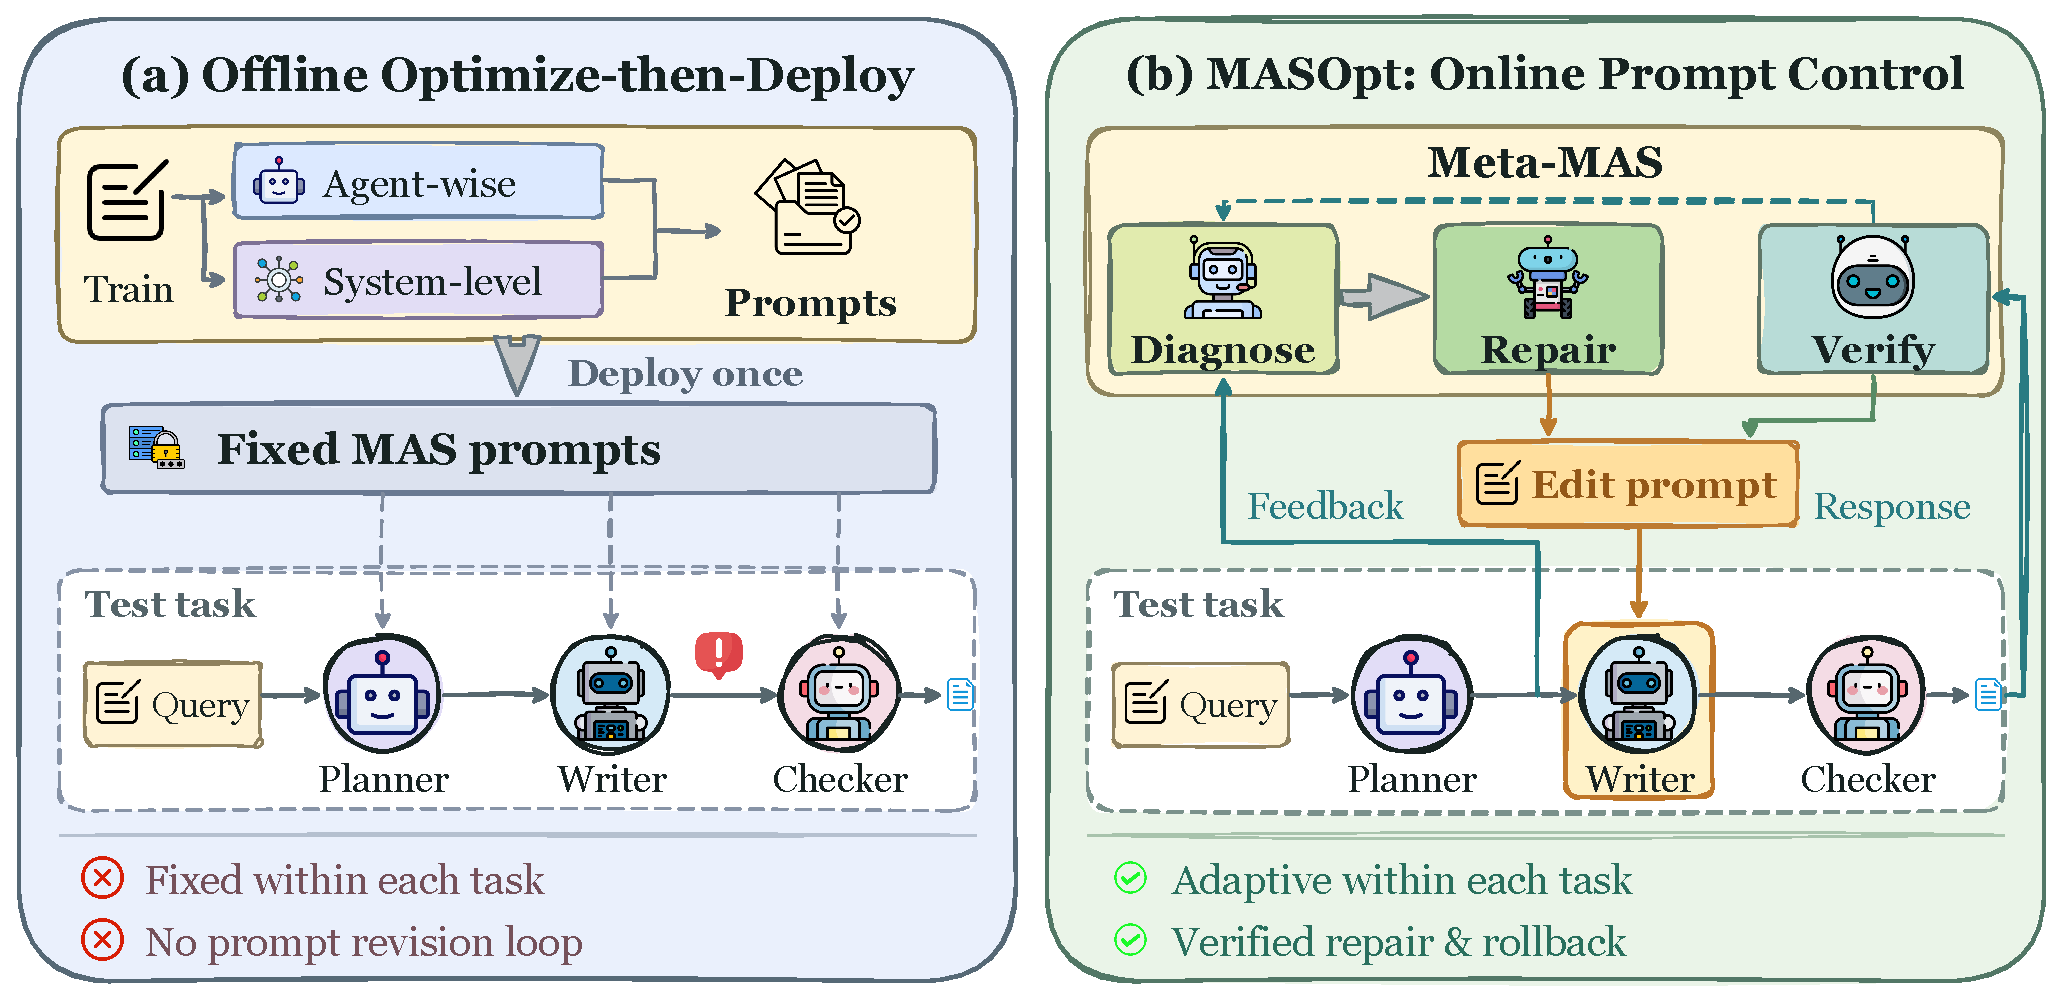
\includegraphics[width=\linewidth]{figures/masopt_introduction_comparison.pdf}
    \caption{Offline prompt optimization and online closed-loop prompt control. \textbf{Left:} agent-wise and system-level optimizers produce a prompt configuration before deployment; that configuration remains largely fixed during a new task. \textbf{Right:} MASOpt uses a Diagnose--Repair--Verify meta-MAS to adapt prompts within the current task. Runtime feedback motivates a local intervention, and its observed effects determine whether to retain or roll back the change; residual feedback drives another round. The task and agent roles are illustrative.}
    \label{fig:masopt-paradigms}
\end{figure}

Online prompt optimization introduces a different challenge.
An intermediate trajectory may reveal that the system has deviated from a desirable behavior, but it does not directly specify how its prompts should be changed.
More importantly, a plausible prompt modification is not necessarily a correct one.
It may resolve the current error, have little effect, or introduce a new downstream failure.
This observation motivates us to view online prompt optimization through the lens of \textbf{closed-loop control theory}
\citep{astrom2008feedback,goodwin2001control}.
A closed-loop controller does not assume that a control action is correct in advance.
It applies an action, observes the resulting system response, and uses the new feedback to determine the next action.
We adopt the same principle for MAS prompt optimization.
Each prompt modification is regarded as a temporary control action.
Its value is determined only after observing how the target MAS responds to the modification.
Successful changes can be retained, harmful ones can be reverted, and partially resolved failures can generate new feedback for another optimization round.

Based on this view, we propose \textbf{MASOpt}, an online prompt optimization framework for multi-agent systems.
MASOpt places a lightweight meta-MAS around a running target MAS.
A \textbf{Diagnose Agent} interprets partial execution trajectories and converts observable failures into structured feedback.
A \textbf{Repair Agent} uses this feedback to construct a minimal local prompt intervention.
A \textbf{Verify Agent} evaluates the post-intervention behavior and determines whether the modification should be retained, reverted, or further refined.
To make this online process efficient, we additionally introduce \textbf{Cross-Actuation Relative Advantage (CARA)}.
During offline calibration, CARA compares alternative prompt interventions from the same execution checkpoint and estimates which types of repairs are more effective under different failure states.
The resulting experience is stored as reusable feedback-control memory and serves as a prior during online optimization.
The target LLMs and MAS topology remain unchanged throughout this process.
MASOpt therefore combines offline repair experience with online closed-loop feedback without requiring model-parameter updates.
Figure~\ref{fig:masopt-paradigms} contrasts this within-task adaptation with offline optimize-then-deploy prompting.

Our contributions are summarized as follows.
\begin{itemize}
    \item \textbf{Online MAS prompt optimization.}
    We introduce, to our knowledge, the first systematic formulation of online prompt optimization for multi-agent systems.
    Unlike conventional optimize-then-deploy approaches, MASOpt allows intermediate execution feedback from the current task to directly modify the prompts used by the remainder of the same task.

    \item \textbf{Closed-loop prompt control with CARA.}
    We formulate online MAS prompt optimization from the perspective of closed-loop control theory and develop a three-agent meta-MAS for diagnosis, repair, and verification.
    We further introduce Cross-Actuation Relative Advantage to learn state-conditioned repair preferences from matched execution states without updating the underlying LLM parameters.

    \item \textbf{Evaluation framework.}
    We specify an evaluation protocol spanning question answering, code generation, mathematical reasoning, and interactive decision-making tasks.
    The protocol isolates the contributions of online verification, matched-state probing, and CARA while avoiding unsupported performance claims before the benchmark runs are complete.
\end{itemize}
